\begin{figure*}	
	\centering
	%\begin{subfigure}[b]{\textwidth}
        %\centerline{
	%  \includegraphics[width=1\textwidth]{images/seed-kraken_plt1_bioinfo_type_HMPtongue_nospans-crop.pdf}
        %}
        %\end{subfigure}
        %
        %\begin{subfigure}[b]{\textwidth}
        %\centerline{	  
	%  \includegraphics[width=1\textwidth]{images/seed-kraken_plt1_bioinfo_type_MiSeq_nospans-crop.pdf}
        %}
        %\end{subfigure}        
        
        \centerline{	  
	  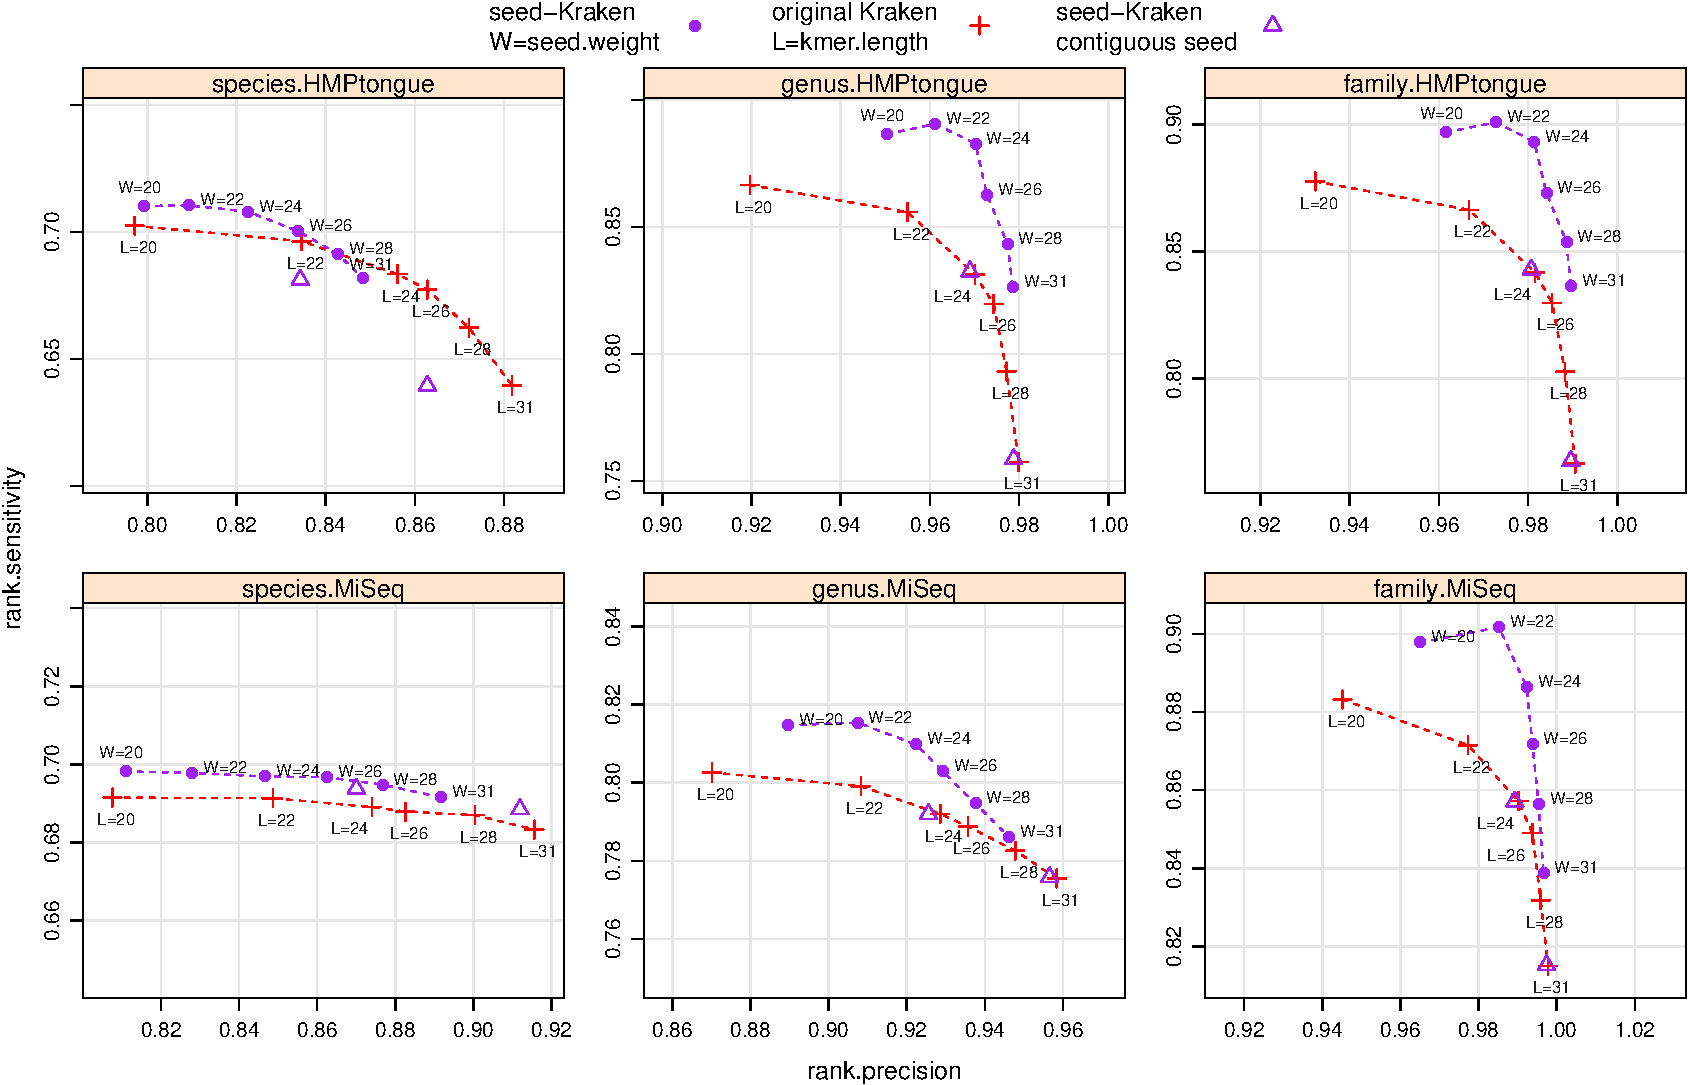
\includegraphics[width=1\textwidth]{images/seed-kraken_plt1_bioinfo_type_HMPtongue_MiSeq_nospans-crop.pdf}
        }                
%	\begin{subfigure}[b]{\textwidth}
%       \centerline{
%	  \includegraphics[width=1\textwidth]{images/seed-kraken_plt1_bioinfo_type_HMPtongue_MiSeq_nospans.pdf}
%      }
%     \end{subfigure}
	\caption{
	 {\revise
Sensitivity/precision  of {\sc seed-Kraken} (circle points) and
original {\sc Kraken} (cross points) 
for HMPtongue and MiSeq datasets and three taxonomic levels: species,
genus and family.
	 % Classification performance of {\sc seed-Kraken} and original {\sc Kraken} 
	 % %Results (receiver operating characteristic - ROC) 
	 % from read classification experiments, which were conducted on 3 data sets HiSeq, MiSeq, HMPtongue. 
	 % Classification sensitivity 
	 % (rate of correct assignments)%(correctly classified/all reads to be classified), 
	 % and precision 
	 % (positive predictive value) %(correctly classified/all attempted classifications), 
	 % was measured at 3 taxonomic levels: family, genus, species.
         % Color filled circles present our selection of (approximately) best performing seeds,
         % which are characterized by weights (indicated), and spans (29 to 42, not indicated). 
         % 
         Triangle points correspond to {\sc seed-Kraken} 
         run on contiguous seed of weight 24 and 31, plotted to highlight the effect of the 
         change in the assignment algorithm. 
%         to indicate the effect of using a slightly different assignment algorithm than {\sc Kraken}.	
	 }
	 %   
%	Classification performance of {\sc seed-Kraken} 
%	and original {\sc Kraken} on three simulated metagenomes HiSeq,
%% (10 bacterial genomes, low error rate), 
%MiSeq 
%% (10 bacterial genomes, average error rate), 
%and simBA-5.
%% (607 bacterial genera, high error rate). 
%Charted are genus precision (positive predictive value) against genus
%sensitivity (rate of correct assignments) depending on seeds, which are characterized by weights (indicated), and spans (31 to 38, not indicated). 
%% Varying are $k$-mer length, and its spaced seed equivalent seed weight, while the seed span is kept constant at $31$. {\sc seed-Kraken} consistently outperforms original {\sc Kraken} in sensitivity/sensibility trade off.
	}
	\label{fig:kraken-experiments}
\end{figure*}
